\chapter{Sensors}
In this chapter, the setup of the sensors used by the segway is described. In a control system the sensors measure the output of the system, $Y$, and feed it back into the system as seen in \autoref{fig:modelBlockS}.

\begin{figure}[H]
\centering
\scalebox{0.8}{
\input{figures/modelBlock.poul}
}
\caption{Feedback loop of a system, with the sensor, $H$, highlighted.}
\label{fig:modelBlockS}
\end{figure}
A general feedback loop, see \autoref{fig:modelBlockS}, consists of three blocks. A controller, $D$, the system that is to be controlled, known as the plant, $G$, and sensors, $H$. The loop holds a reference signal, $R$, an error signal, $E$, the control signal, $U$, between the controller and the plant, and an output, $Y$. It is the sensor block, that is to be determined in this chapter, as highlighted in \autoref{fig:modelBlockS}.

In Section \ref{controlLoopOverview}, it was argued why the transfer function of the sensor block was set to be equal to 1, i.e. $H(s)=1$. Even though this is the case, the sensors used in the system still need to be described, so it is known which parameters of the system are measurable. This is also important to investigate since the way the data is obtained might influence the implementation of the controller.

The segway has four sensors that can be used to measure the speed, angular velocity and angle of the segway. To measure the speed, two encoders are available to measure the rotational velocity for both motors. The angle and angular velocity can be found from the gyroscope and the accelerometer. The structure of the following sections is to first describe the interface between the sensor hardware and the microcontroller (MCU) ATxmega128A3U and afterwards explain the implementation. %How the data is preprocessed is also described. The implementation is done on a ATxmega128A3U microprocessor. 

\section{Accelerometer and Gyroscope}
From \autoref{sec:hardware} it is known that the accelerometer and gyroscope are part of the MPU6050 transducer. This sensor has six degrees of motion, since both the accelerometer and gyroscope are 3-axis sensors. The accelerometer and gyroscope are used to derive the angle and angular velocity of the segway. To acquire the measured data from the sensors, the sensors have an \gls{I2C} bus, which can be interfaced to from the MCU.
  
\subsection{\iic Data}
The physical interface consists of two wires Serial Data (SDA) and Serial Clock (SCL). In normal mode the bus supports clock speeds up to 400 kHz, but additions can be made so the speed can go up to 5 MHz \citep{I2C}. In idle the voltage on the data line is pulled high. On a data level, a transmission consists of a start sequence, 7 bit address, R/W bit, acknowledge, followed by a start sequence, 8 data bit, acknowledge and a stop sequence. This can also be seen in \autoref{fig:I2CFrame}. Note that it is possible to transmit multiple data bytes without having to specify the address between each data transfer.

\begin{figure}[H]
\centering
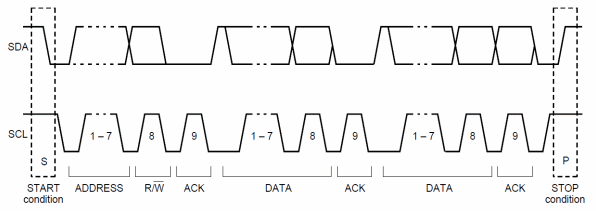
\includegraphics[width=\textwidth]{I2Cframe.png}
\caption{A visual representaion of a \gls{I2C} frame \citep{sou:i2c}.}
\label{fig:I2CFrame}
\end{figure}

\subsection{Data Acquisition from Gyroscope and Accelerometer}
The \gls{I2C} communication protocol is implemented in the MCU as a software module, since the pins, connected to pin 0 and 1 on port A, do not support hardware \gls{I2C}. The implemented \gls{I2C} driver, has been provided by group 15gr633, from AAU, who previously worked with the segway. From the header file, it can be seen that the library has 11 functions \autoref{lst:I2CFunctions}. From these functions the three functions i2cInit, i2cWrite and i2cRead are the main functions, the rest are subroutines that are called from the main functions.

\lstset{language=C, caption={Pre initialization of \gls{I2C} functions.}, label=lst:I2CFunctions}
\begin{lstlisting}
void i2cInit();
uint8_t i2cWrite(uint8_t slaveAddr, uint8_t regAddr, uint8_t *data, uint8_t length);
uint8_t i2cRead(uint8_t slaveAddr, uint8_t regAddr, int8_t *data, uint8_t length);

void i2cRepeatedStart(); 
void i2cStart();
void i2cStop();
void i2cTransmit(uint8_t data);
uint8_t i2cReceive();
uint8_t i2cGetAck();
uint8_t i2cSendAck();
uint8_t i2cSendNack();
\end{lstlisting}

From the datasheet it is known that the MPU6050 sensors \gls{I2C} address is 0x68 \citep[p. 46]{gyro}. When the sensor is powered on, it is in sleep mode. To wake up the sensor, 0x00 is written to the PWR\_MGMT\_1(Power Management 1) 8-bit register. Each sensor has six 8-bit registers for measured data. The three axes' values are sampled by three 16-bit ADC and then stored as MSB and LSB, giving six data registers for each sensor. From the datasheet it is known that the accelerometer data is stored in the registers from 0x3B to 0x40, while the gyroscope data is stored in the registers from 0x43 to 0x48. 

Note that both the gyroscope and the accelerometer work in polling mode, meaning that the current measurements are not sent automatically to the microcontroller, but will instead have to be requested over \gls{I2C}. The sensor modules takes care of obtaining the measurements and storing them in an internal register automatically - it is only the extraction of this data that is done in polling mode.

\subsection{Data Processing the Gyroscope and Accelerometer}
When the data is collected from the registers, they are put together to three 16 bit words. The accelerometer and gyroscope use the same coordinate system, but the orientation of this coordinate system (x, y, z) must be compared to the segway, which can be seen in \autoref{fig:sensor_orientation}. 

\begin{figure}[H]
\centering
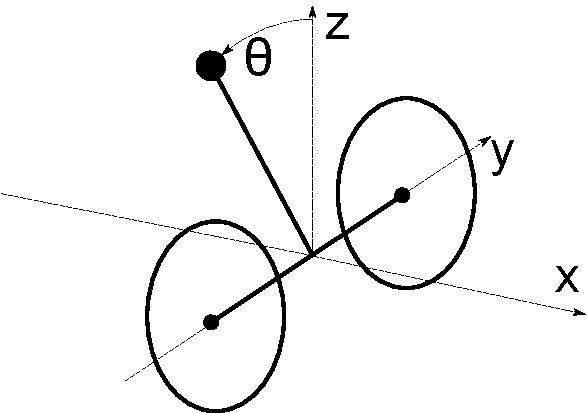
\includegraphics[width=0.4\textwidth]{figures/3D_seg_balance.pdf}
\caption{The sensors' orientation compared to the segway.}
\label{fig:sensor_orientation}
\end{figure}

To calculate the tilting angle of the pendulum, $\theta_p$, different methods can be used. For instance, the accelerometer can calculate the angle based on the direction of gravity, or by integrating the gyroscope data, which measures angular velocity. These methods have a couple of problems though. For instance, the accelerometer is very sensitive to changes in movement due to the acceleration applied. The gyroscope however, has a tendency to drift due to the integration \citep{IMU}. To obtain the angle it can therefore be advantageous to combine these measurements. This is done in a complementary filter \citep{IMU}, where measurements from both of the sensors are weighted and summed. 
\newpage
From \autoref{fig:sensor_orientation} it can be deducted that the pendulum angle can be calculated based on the accelerometer as: 
$$\theta_{pAx} = -\text{tan}^{-1}\left(\frac{x_{Ax}}{z_{Ax}}\right)$$ 
\begin{where}
\va{$\theta_{pAx}$}{is the angle of pendulum}{$\text{rad}$}\\
\va{$x_{Ax}$}{is the accelerometer measurement in the x-axis}{1}\\
\va{$z_{Ax}$}{is the accelerometer measurement in the z-axis}{1}\\
\end{where}

To get the angular velocity from the gyroscope, it is first recognised, based in \autoref{fig:sensor_orientation}, that it is the data in the y-axis, that is of interest. 
The angular velocity can then be calculated as follows:
\begin{equation}
\omega_p = \frac{y_{Gyro} \cdot max}{n}
\end{equation}
\begin{where}
	\va{$\omega_p$}{is the angular velocity of the pendulum}{rad/s}
	\va{$y_{Gyro}$}{is the data from the gyroscope in the y-axis}{1}
	\va{$max$}{is the gyroscope maximum measurement}{rad/s}
	\va{$n$}{is the number of digital representation for the gyroscope data}{1}
\end{where}

Using the complementary filter, the angle can be found as:

\begin{equation}
\theta_p = k \cdot \theta_{pAx} + (1-k) \cdot \int \!\omega_p \,\rm{d}x
\label{complementary}
\end{equation}

From \autoref{complementary}, it is seen how the angle is estimated from both accelerometer and integrated gyroscope data, and then the two values are weighted. The weighting factor $k$ is found experimentally to 0.05.
\newpage
\section{Encoder and Quadrature Decoder}

To determine the velocity of the wheels at a specified time, the exact change of position over an infinitesimal timespan shall be known, as the velocity $v(t)$ can be expressed by the time derivative of the position $s(t)$:
\begin{align}
v(t) = \frac{\text{d}s(t)}{\text{d}t}
\label{velocity}
\end{align}
\begin{where}
\va{$v(t)$}{is a function for velocity}{$\text{m/s}$}\\
\va{$s(t)$}{is a function for position}{$\text{m}$}\\
\end{where}

To determine a function for the position it is desired to decode the output signal from the encoders since they provide measurements about position changes over time. 

The encoders used for the segway are quadrature encoders. The output from a quadrature encoder is two square waves phase shifted by 90$\degree$ from two channels as illustrated in \autoref{fig:incremental_encoders2}. 

\begin{figure}[H]
	\centering
	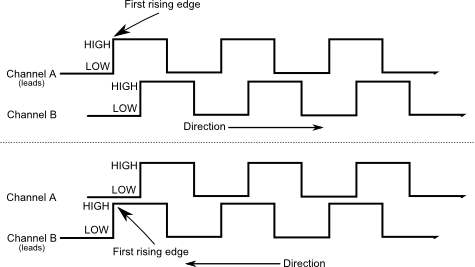
\includegraphics[width=0.7\textwidth]{figures/quad-encoding-waveform.png}
	\caption{Quadrature signal \citep{sou:quad_enc}.}
	\label{fig:incremental_encoders2}
\end{figure}

The signals from the encoders provide information about the direction and velocity of the wheel. Since the square waves from channel A and B are 90$\degree$ out of phase, the direction of the wheels can be found by determining the first rising edge of the signals from channel A and B. As the direction of the wheels change, the first rising edge will occur at the other channel.

The velocity can be determined by the number of of the square waves per time unit. One encoder rotation correspond to 512 high/low cycles or 2048 counts. A count is an event change in either channel A or B. E.g. if channel A goes low it will result in a count. The relation between the position and the number of counts is given by:

\begin{align}
s(t) = \frac{d \cdot \pi \cdot N_{ms} \cdot N_{sw}}{4\cdot CPR} \cdot c(t) \qquad \{c(t) \in \mathbb{Z}\}
\end{align}
\begin{where}
\va{$d$}{is the diameter of the wheel}{$\text{m}$}\\
\va{$N_{ms}$}{is the encoder/shaft ratio}{1}
\va{$N_{sw}$}{is the shaft/wheel ratio}{1}
\va{$c(t)$}{is number of counts. $c(t)$ can only be an integer.}{1}
\va{$CPR$}{number of cycles in one encoder rotation}{1}
\end{where}

The function $c(t)$ changes by the velocity of the wheels. Since $c(t)$ is an integer, the resolution of the position change is limited to the a-coefficient in the equation of $s(t)$, which is a linear expression on the form $s(t) = a \cdot c(t)$. The a-coefficient can be calculated by inserting the values given by the datasheets and measurements, see \autoref{app:segwayParameters} and \autoref{motorMeasReport}.
\begin{align}
s(t) = \frac{d \pi \cdot N_{ms} \cdot N_{sw}}{4\cdot CPR} \cdot c(t) \Rightarrow s(t) = \frac{0.117 \, \text{m} \cdot \pi \cdot  \frac{1}{19} \cdot \frac{25}{90}}{4\cdot 512} \cdot c(t) \approx 2.62 \cdot 10^{-6} \: \text{m} \cdot c(t)
\label{eq_st}
\end{align}

\autoref{eq_st} yields that 1 count is equal to $2.62 \cdot 10^{-6} \: \text{m}$. The expression of $s(t)$ from \autoref{eq_st} is inserted into \autoref{velocity}, yielding:
\begin{align}
v(t) = 2.62 \cdot 10^{-6} \: \text{m} \cdot \frac{\text{d}c(t)}{\text{d}t} \qquad \{c(t) \in \mathbb{Z}\}
\label{eq_vel}
\end{align}

Since the microcontroller responsible for measuring the encoder only works in discrete time, it is impossible to compute the derivative in \autoref{eq_vel}. Instead, a close approximation of \autoref{eq_vel} can be described as:
\begin{align}
v(t) \approx 2.62 \cdot 10^{-6} \: \text{m} \cdot \frac{c(t)-c(t_1)}{t-t_1} = 2.62 \cdot 10^{-6} \: \text{m} \cdot \frac{\Delta c(t)}{\Delta t}
\label{eq_vel2}
\end{align}

Whereas \autoref{eq_vel} gives the exact velocity of the wheels at a given time $t$, \autoref{eq_vel2} gives the approximated velocity in the time span $\Delta t$. This means the precision of the velocity is determined by $\Delta t$. A smaller time span $\Delta t$ gives a better precision.
If the time span $\Delta t$ is fixed, meaning $\Delta t$ is always set to 1 ms, the time span can known as the sampling period $T_{s}$. The inverse of $T_{s}$ is the sampling frequency $f_{s}$.
\begin{align}
v(t) \approx 2.62 \cdot 10^{-6} \: \text{m} \cdot f_s \cdot \Delta c(t) 
\end{align}

To get an accurate velocity, the sampling frequency is set to 1 kHz, but due to rounding in the frequency scaling in the MCU, this frequency cannot be obtained exactly. This small error is however disregarded.
\begin{align}
v(t) \approx 2.62 \cdot 10^{-6} \: \text{m} \cdot 1 \: \text{kHz} \cdot \Delta c(t)  = 2.62 \cdot 10^{-3} \: \frac{\text{m}}{\text{s}} \cdot \Delta c(t) 
\label{eq_vel3}
\end{align}

From this, the wheel angular velocity can also be found:
\begin{align}
\omega_w(t) = \frac{2\pi}{r_w}\cdot v(t) = 963 \cdot 10^{-6} \cdot \Delta c(t) \frac{\text{rad}}{\text{s}}
\end{align}	
The next step is to implement \autoref{eq_vel3} on the microcontroller.

\subsection{Quadrature Decoder Setup}
To process the data from the encoders, some decoders are needed. As stated previously, every event equals to a logical change from channel A or B from the encoders. Since the segway features two encoders, one encoder is connected to port C and another to port E. To allow event detection on the XMEGA, the registers associated with the quadrature decoding are set. The functions used for the setup of the quadrature decoders are seen in \autoref{lst:encoderFunctions}.

\lstset{language=C, caption={Pre-initialization of quadrature decoder functions.}, label=lst:encoderFunctions}
\begin{lstlisting}
void qdec_setup();			// Setup registers for the quadrature decoder
void en_interrupt();		// Enable interrupt
float motor_speed_left();	// Calculate and return the velocity of the left wheel
float motor_speed_right();
\end{lstlisting}

All registers associated with the quadrature decoders are set in the function qdec\_setup(), where the hardware for the decoder is set up. The XMEGA has external hardware that supports quadrature decoding. This means that the microprocessor does not directly need to handle the encoder itself, but only needs to read the data from the decoder through an interrupt service routine (ISR). After calling this function, a counter register will increment by one every time an event changes is occurring from channel A and B from both encoders. 

\subsection{Data Processing the Encoder Measurements}
As previously stated, the sampling frequency for the decoders are set to $f_s = 1$ kHz. To ensure a sampling every 1 ms, a timer is set to count up 1 ms and interrupts in order to sample the counter from the decoders. The interrupt service routine is seen in \autoref{lst:decoderISR}.

\lstset{language=C, caption={Interrupt Service Routine (ISR) for sampling the counters.}, label=lst:decoderISR}
\begin{lstlisting}
ISR(TCD1_OVF_vect){
	encoder_ccnt = TCC1.CNT;		// Get the value from port C counter register
	encoder_ecnt = TCE1.CNT;		// -||- port E
	TCE1.CNT = 0;					// Reset the counter register
	TCC1.CNT = 0;									
}
\end{lstlisting}
If the velocity of the wheels is required, the functions motor\_speed\_left() and motor\_speed\_right() are called. The functions then return the speed of the left and right wheel. This is done by converting the encoder counter to velocity using \autoref{eq_vel3}.
%\begin{equation}
%	\omega_w = 2 \cdot \pi \cdot f_s \cdot N_{ms} \cdot N_{sw} \cdot \frac{cnt}{4 \cdot res}
%\end{equation}
%\begin{where}
%\va{$\omega_w$}{is the angular velocity of the wheel}{rad/s}\\
%\va{$f_s$}{is the sampling frequency of the encoders}{Hz}\\
%\va{$N_{ms}$}{is the gearing ratio from the motor to the shaft}{1}\\
%\va{$N_{sw}$}{is the gearing ratio from the shaft to the wheel}{1}\\
%\va{cnt}{is the counted value for the specific encoder}{1/RPM}\\
%\va{res}{is the resolution of the encoders}{1/RPM}
%\end{where}

\section{PWM and H-bridge}
To control the DC-motors connected to the wheels, two H-bridges are used. By using H-bridges it is possible to control both the direction and the speed of the DC motors. For each H-bridge, the pins D2, IN1 and IN2 on the H-bridge are used for this purpose. By feeding D2 with a PWM signal, the velocity is changed by changing the duty cycle. A duty cycle of 100\% results in the motors going on full speed, whereas a duty cycle of 0\% results in no rotation. To determine the direction, either IN1 or IN2 should be pulled high. \\\\
The H-bridges' IN1 and IN2 pins are connected to the microcontroller's pin PC2 and PC3, and PE2 and PE3. The D2 pin is connected to PC1 and PE1 - these pins are set to be the PWM generating outputs in the MCU. The functions associated with PWM generation can be seen in \autoref{lst:pwmFunctions}.

\lstset{language=C, caption={Pre initialization of PWM generation functions.}, label=lst:pwmFunctions}
\begin{lstlisting}
void PWM_setup();
void PWM_left(int duty);
void PWM_right(int duty);
\end{lstlisting}

When generating a PWM signal, the resolution of the PWM signals are set to 256 counts, which is considered to be sufficient.\\
As the sensor block in the feedback loop, see \autoref{fig:modelBlockS}, is now known, the system model of the segway is to be derived in the following chapter. 


%\section{Controllers}
